\chapter{Scattering Theory}\label{chap:3}
\section{Two-body Scattering} \label{Two-body scattering}
A collision between a pair of particles can be described in their centre-of-mass frame as the scattering of a particle with reduced mass $\mu_{2\mathrm{b}}$ ($\mu_{2\mathrm{b}} = m_1m_2/(m_1 + m_2)$) by the potential $V(\mathbf{r})$. The time-independent  Schr{\"o}dinger equation for the relative motion is then given by 

\begin{equation} \label{eq:22}
\bigg[-\frac{\hbar^2}{2\mu}\nabla^2 + V(\mathbf{r})\bigg]\psi(\mathbf{r}) = \frac{\hbar^2 k^2}{2 \mu}\psi(\mathbf{r}),
\end{equation}
where $\mathbf{r}$ denotes the interparticle separation and $\nabla^2$ the Laplace operator, which in spherical coordinates reads

\begin{equation} \label{eq:23}
\nabla^2 = \frac{1}{r^2} \frac{\partial}{\partial r} \bigg(r^2 \frac{\partial}{\partial r}\bigg) + \frac{1}{r^2 \sin\theta} \frac{\partial}{\partial\theta} \bigg(\sin\theta \frac{\partial}{\partial\theta}\bigg) + \frac{1}{r^2 \sin^2\theta} \frac{\partial^2}{\partial\phi^2}.
\end{equation}
By requiring the potential to be zero at large interparticle separation, the collision can be described as that of an incident plane wave with definite angular momentum that scatters off a potential placed at the origin. The potential will deflect some of the incident waves to form scattered waves, which at large distances will be diverging from a point source in the scattering region. Let $r_0$ denote the range of the action of the potential and let $z$ denote the direction of the propagation of the incident plane wave. The boundary condition at large separations $r \gg r_0$ then imposes a solution of the following asymptotic form

\begin{equation}\label{eq:26}
\psi(\mathbf{r}) \xrightarrow{r \to \infty} e^{ikz} + f(k,\theta,\phi)\frac{e^{ikr}}{r},
\end{equation}
in which the total wave function is written as a superposition of the incident and scattered wave, with a scattering amplitude $f(k,\theta,\phi)$ that depends on the energy of the particle through $k$, the deflection angle $\theta$ between the waves and the azimuthal angle $\phi$ about the $z$-axis. For spherically symmetric potentials, i.e., $V(\mathbf{r}) = V(r)$, the Schr{\"o}dinger equation \eqref{eq:22} is separable. The incident and scattered wave functions are then conveniently expanded on a basis set of eigenfunctions of $\mathbf{L}^2$ and $L_z$, where $\mathbf{L}$ is the relative orbital angular momentum operator. These eigenfunctions are the spherical harmonic functions $Y_l^m(\theta,\phi)$, which satisfy 

\begin{equation}
\mathbf{L}^2 Y_l^m(\theta,\phi) \equiv -\frac{1}{ \sin^2\theta} \bigg[ \sin\theta \frac{\partial}{\partial\theta} \bigg(\sin\theta \frac{\partial}{\partial\theta}\bigg) +  \frac{\partial^2}{\partial\phi^2}\bigg] Y_l^m(\theta,\phi) = l(l+1)Y_l^m(\theta,\phi).
\end{equation}
The most general solution to \Cref{eq:22} is then of the form

\begin{equation}\label{eq:32}
\psi(\mathbf{r}) = \sum_{l=0}^{\infty} \sum_{m = -l}^{l} C_{lm}\frac{u_{l}(r)}{r}Y_l^m(\theta,\phi).
\end{equation}
The separability of $\psi(\mathbf{r})$ effectively reduces the problem to that of solving the radial equation

\begin{equation} \label{eq:24}
\bigg[-\frac{d^2}{dr^2} + \frac{l(l+1)}{r^2} + \frac{2\mu}{\hbar^2}V(r) - k^2\bigg]u_l(r) = 0.
\end{equation}
By requiring the wave function to be finite  everywhere it is implied that $u_l(r)$ must vanish at the origin. In the case where $V(r) = 0$, the solutions to the radial equation for positive energies have the form

\begin{equation}\label{eq:zero}
u_l(r) \propto r j_l(kr),
\end{equation}
where $j_l(kr)$ are the spherical Bessel functions. In the case of a non-zero potential the solutions need to be regular at the origin, while at large distances $r \gg r_0$ they have the form

\begin{equation}\label{eq:25}
u_l(r) = r(a_l j_l(kr)+b_l y_l(kr)),
\end{equation} 
where $y_l(kr)$ are the spherical Neumann functions. Asymptotically the solutions \Cref{eq:25} behave like

\begin{equation}
u_l(r) \xrightarrow{r\to\infty} \frac{1}{k}\big(a_l \sin(kr - l\frac{\pi}{2})-b_l \cos(kr - l\frac{\pi}{2})\big).
\end{equation} 
By defining the ratio of the coefficients as

\begin{equation}\label{eq:tan}
\frac{b_l}{a_l} = -\tan\delta_l(k),
\end{equation} 
where $\delta_l(k)$ is an energy dependent phase shift, the normalized asymptotic radial solutions for a non-vanishing potential can be written

\begin{equation}\label{eq:assympt}
\begin{split}
u_l(r) \xrightarrow{r \to \infty} &\frac{1}{k}\big(\sin(kr - l\frac{\pi}{2} + \delta_l(k))\big)\\
=&\frac{e^{-i\delta_l(k)}}{2ik}\big((-1)^{l+1}e^{-ikr} + e^{2i\delta_l(k)}e^{ikr}\big).
\end{split}
\end{equation}
Since the incident plane wave in \Cref{eq:26} is aligned with the $z$-axis, it is an eigenfunction of $L_z$ with an eigenvalue $m=0$. The plane wave expansion is thus independent of the azimuthal angle around the $z$-axis and can therefore be expressed as

\begin{equation}\label{eq:27}
e^{ikz} = \sum_{l=0}^{\infty} (2l+1)i^l j_l(kr)P_l(\cos\theta),
\end{equation}
where $P_l(\cos\theta)$ are the Legendre polynomials. It is evident that this plane wave is a solution to \Cref{eq:22} for $V(r) = 0$, and in the asymptotic limit these solutions behave like

\begin{equation}\label{eq:29}
e^{ikz} \xrightarrow{r \to \infty} \frac{1}{2ikr} \sum_{l=0}^{\infty} (2l+1)P_l(\cos\theta)\big((-1)^{l+1}e^{-ikr} + e^{ikr}\big).
\end{equation}
The incident plane wave can thus be resolved into that of incoming ($e^{-ikr}$) and outgoing ($e^{ikr}$) spherical waves with a relative phase of $0$ for $l$ with odd parity and of $\pi$ otherwise. Substituting \Cref{eq:29} into \Cref{eq:26} results in an asymptotic wave function of the form

\begin{equation}\label{eq:30}
\psi(\mathbf{r}) \xrightarrow{r \to \infty} \frac{1}{2ikr}\sum_{l=0}^{\infty} (2l+1)P_l(\cos\theta))\big((-1)^{l+1}e^{-ikr} + e^{ikr}\big) + f(k, \theta) \frac{e^{ikr}}{r},
\end{equation} 
where the scattering amplitude $f(k,\theta,\phi)=f(k,\theta)$ because the scattering potential is spherically symmetric. Since the system is rotationally invariant about the $z$-axis, the scattered wave function must be azimuthally symmetric, i.e., have a magnetic quantum number $m=0$, wherefore the general solution to \Cref{eq:32} becomes

\begin{equation}\label{eq:28}
\psi(\mathbf{r}) = \sum_{l=0}^{\infty} c_l \frac{u_l(r)}{r} P_l(\cos\theta),
\end{equation} 
in which $c_l$ are unknown coefficients. The asymptotic behaviour of \eqref{eq:28} is thus

\begin{equation}\label{eq:31}
\psi(\mathbf{r}) \xrightarrow{r \to \infty} \frac{1}{2ikr} \sum_{l=0}^{\infty} c_l P_l(\cos\theta) e^{-i\delta_l(k)} \big((-1)^{l+1}e^{-ikr} + e^{2i\delta_l(k)}e^{ikr}\big).
\end{equation} 
By comparing the asymptotic form of the incoming waves expressed in \cref{eq:30,eq:31} it is evident that the coefficients $c_l = (2l+1)e^{i\delta_l(k)}$, and the asymptotic scattered wave is therefore given by

\begin{equation}\label{eq:33}
\psi(\mathbf{r}) \xrightarrow{r \to \infty} \frac{1}{2ikr} \sum_{l=0}^{\infty} (2l+1) P_l(\cos\theta)\big((-1)^{l+1}e^{-ikr} + e^{2i\delta_l(k)}e^{ikr}\big).
\end{equation}
For elastic scattering the flux of incoming and outgoing waves is conserved. The presence of a scattering potential will modify the plane wave by changing the relative phase of the incoming and outgoing waves by a phase shift $\delta_l(k)$ for each partial wave with angular momentum $l$. The phase shift $\delta_l(k)$ is thus a measure of the distortion of $u_l(r)$ from the free solution due to the presence of a scattering potential. Depending on whether the potential is attractive or repulsive, the scattered wave will either be pulled in or pushed out, respectively, by the scatterer. The scattering amplitude $f(k,\theta)$ is determined by comparing the outgoing waves in \cref{eq:30,eq:33}, resulting in

\begin{equation}
f(k,\theta) = \sum_{l=0}^{\infty} (2l+1)f_l(k)P_l(\cos\theta),
\end{equation}
where the partial amplitude $f_l$ can be expressed in the following ways

\begin{equation}\label{eq:partialamp}
f_l(k) = \frac{e^{2i\delta_l(k)}-1}{2ik} = \frac{e^{i\delta_l(k)}\sin\delta_l(k)}{k} = \frac{1}{k\cot\delta_l(k) - ik}. 
\end{equation}
The differential and the total cross-sections are determined from the scattering amplitude through 

\begin{equation}
\frac{d\sigma}{d\Omega}=\abs{f(k,\theta)}^2,
\end{equation}
and

\begin{equation}
\sigma(k)= \sum_{l=0}^{\infty} \sigma_l(k) = \frac{4\pi}{k^2}\sum_{l=0}^{\infty}(2l+1)\sin^2\delta_l(k),
\end{equation}
in which $\sigma_l$ is the scattering cross-section for each partial wave. So far, we have assumed that the particles are distinguishable and that scattering in the direction $\theta$ could be discriminated from that of scattering in the direction $\pi-\theta$. However, for identical particles these collisional processes will lead to the same final state. Interchanging the spatial coordinates of the particles $\mathbf{r}_1 \leftrightarrow \mathbf{r}_2$ corresponds to replacing the relative position vector $\mathbf{r}$ by $-\mathbf{r}$, which in polar coordinates corresponds to replacing ($r,\theta,\phi$) by ($r,\pi-\theta,\phi+\pi$). Thus, to accurately describe scattering of identical particles the quantum statistics of the particles must be taken into account to assure that the wave function of the total system has the correct symmetry properties. The wave function given in \Cref{eq:26} does, however, not fulfill this requirement. Instead, the correct two-body wave function in the centre-of-mass frame for indistinguishable particles is retrieved by symmetrization (bosons, $\epsilon = 1$) or antisymmetrization (fermions, $\epsilon = -1$), leading to

\begin{equation}
\psi(\mathbf{r}) \xrightarrow{r \to \infty} \frac{e^{ikz} + \epsilon e^{-ikz}}{\sqrt{2}} + \frac{f(k,\theta)+\epsilon f(k,(\pi-\theta))}{\sqrt{2}}\frac{e^{ikr}}{r}.
\end{equation}
In classical mechanics, the differential cross-sections for the two processes described above would simply add up. However, the quantum mechanical differential cross-section for indistinguishable particles is given by

\begin{equation}
\frac{d\sigma}{d\Omega} = \abs{f(k,\theta)+\epsilon f(k,(\pi-\theta))}^2, \quad \text{for} \quad 0 \leq \theta \leq \frac{\pi}{2},
\end{equation}
where the sum of probability amplitudes is

\begin{equation}
f(k,\theta) \pm f(k,(\pi-\theta)) = \frac{1}{2ik}\sum_{l=0}^{\infty} \big[1 \pm (-1)^l\big](2l+1)P_l(\cos\theta)(e^{2i\delta_l(k)} - 1).
\end{equation}
Note that the total cross-section is obtained by integrating over half of the solid angle $\Omega =4\pi$ in the case of identical particles. The expression for the total cross-section for elastic scattering after integration is then

\begin{equation}\label{eq:34}
\sigma(k)=
\frac{8\pi}{k^2}\sum_{l=0}^{\infty} (2l+1)\sin^2\delta_l(k). 
\end{equation}
In the case of bosons, only even values of $l$, and in the case of fermions, only odd values of $l$, will contribute to the total cross-section \eqref{eq:34}.

\section{The Low Energy Limit}
At very low energies, i.e., when the angular de Broglie wavelength $\lambdabar = 1/k$ is much larger than the interparticle interaction range $kr_0 \ll 1$, higher partial waves become unimportant except for potentials that are strong enough to form $l\neq 0$ bound states near the threshold ($E \simeq 0$). This can be understood classically by considering that particles with angular momentum $l$ and energies much lower than the height of the centrifugal barrier, i.e., the angular momentum term in the effective potential $V_{eff} = V(r) + \hbar^2l(l+1)/2\mu r^2$, will simply be reflected by the barrier and only the lowest partial wave $l=0$ will be able to come close enough to be scattered by the potential $V(r)$. For short-ranged two-body interactions, i.e., potentials that fall off faster than $r^{-2}$, the angular momentum term is the potential of the longest range and will thus largely govern the threshold behaviour ($E=0$) of the radial wave function. Since the potential and the $k^2$ term can be neglected in the radial equation \eqref{eq:24} for separations larger than the interaction range $r \gg r_0$, the general solution $R_l = u_l/r$ at threshold is given by

\begin{equation}\label{eq:35}
R_l(E=0) = c_1r^l + c_2r^{-(l+1)}.
\end{equation}
By joining this solution to the asymptotic solution for $E>0$, given in \Cref{eq:assympt} one can show that

\begin{equation}
\tan\delta_l(k) \simeq \delta_l(k) = \frac{c_2}{c_1}\frac{k^{2l+1}}{(2l-1)!!(2l+1)!!} = (-a_lk)^{2l+1},
\end{equation}
in which $a_l$ is the scattering length for the $l$th partial wave. The arguments above form the basis of the Wigner threshold law \cite{Landau1965Quantum,Sadeghpour_2000}, which states that at near threshold, the phase shift goes to zero like

\begin{equation}
\delta_l(k) \propto k^{2l+1} \pmod{\pi} \quad \text{when} \quad k \rightarrow 0.
\end{equation}
The cross-section for that partial wave then approaches zero like

\begin{equation}
\sigma_{l \neq 0}(k) = \frac{8\pi}{k^2}(2l+1)\sin^2\delta_l(k) \propto k^{4l} \quad \text{when} \quad k \rightarrow 0,
\end{equation}
wherefore $s$-wave scattering is dominant for short-ranged potentials in the low energy limit. The only non-zero cross-section is the one for the $s$-wave, which, using \Cref{eq:partialamp}, is given by

\begin{equation}
\sigma = \sigma_0 = 8\pi \lim_{k \to 0} \bigg|\frac{1}{k\cot\delta_0 -ik}\bigg|^2 = 8\pi a^2,
\end{equation}  
in the case of identical bosons ($\sigma = 4\pi a^2 $ for distinguishable particles) and where $a$ is the $s$-wave scattering length, previously defined in \Cref{eq:2}.

\subsection{Zero-energy Scattering}\label{sec:zero_energy_scat}
In the ultracold regime the energy is extremely low and $k\simeq0$. The radial equation simplifies to

\begin{equation}
-\frac{d^2 u_l(r)}{dr^2} + \frac{2\mu}{\hbar^2}V(r)u_l(r) = 0.
\end{equation}
The asymptotic solution for $l=0$ ($u = u_0$) is then

\begin{equation}\label{eq:radzero}
u(r) \xrightarrow{ r \to \infty} \frac{1}{k} \sin\bigg[k\Big(r+\frac{\delta_0}{k}\Big)\bigg]  \xrightarrow{k \to 0} \text{constant}(r-a).
\end{equation}
The logarithmic derivative is given by

\begin{equation}
\frac{u'(r)}{u(r)}  \xrightarrow{ r \to \infty} k \cot\bigg[k \Big(r + \frac{\delta_0}{k}\Big)\bigg] \xrightarrow{k \to 0} \frac{1}{r-a}.
\end{equation}
In the limit $kr \ll 1$, the scattering length is obtained as

\begin{equation}
a = -\lim_{k \to 0} \frac{\tan \delta_0 }{k} = \lim_{k,r \to 0,\infty}\Bigg(r-  \frac{u(r)}{u'(r)}\Bigg).
\end{equation}
From \Cref{eq:radzero} it is evident that the scattering length is simply the radius at which the tangent to the radial wave intercepts the $r$-axis. This concept can be illustrated by using a short-ranged attractive model potential given by

\begin{equation}\label{modelpotential}
V(r) = -\frac{c_w\bigg[1-\Big(1 + \frac{r^2}{r_c^2}\Big)e^{-\frac{r^2}{r_c^2}}\bigg]}{r^6},
\end{equation}
in which $r_c$ and $c_w$ are tuning parameters for the distance to the nadir and the depth of the potential, respectively. The scattering length can be varied by fine-tuning the potential depth, see \Cref{fig:potential_depth}. Starting with an attractive potential with negative scattering length, i.e., with a tangent intercept on the negative side, when increasing the potential depth, the magnitude of the scattering length will increase and as $a \rightarrow -\infty$ the radial wave function will become flat. A further increase in potential depth will cause $a$ to change sign $a \rightarrow \infty$. The sign shift of $a$ is associated with the forming of a bound state. After the change in sign, a further increase in depth will instead correspond to decreasing $a$ since the radial wave function now crosses the $r$-axis on the positive side, with the intercept subsequently approaching the origin, see \Cref{fig:intercept}. This behaviour is then repeated in the same way until a new bound state is formed, see \Cref{fig:scattapp}.

\begin{figure}
	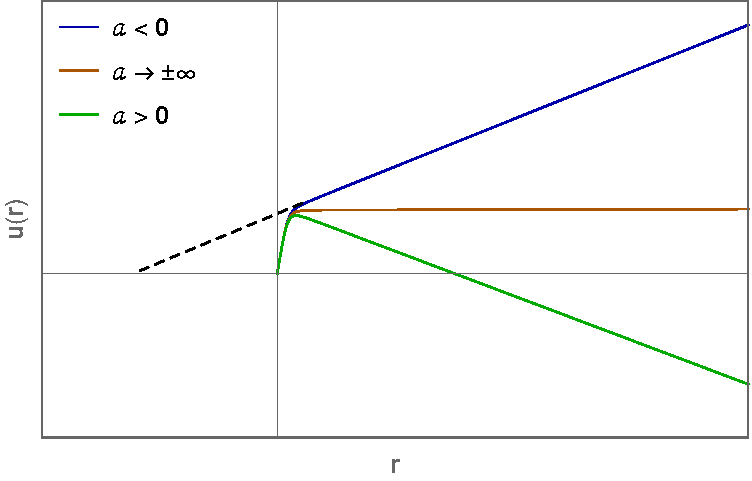
\includegraphics[width=\linewidth]{intercept.pdf}
	\caption{Plot of $u(r)$ versus $r$ for the model potential \eqref{modelpotential} at three different depths. The radius at which the tangent intercepts the $r$-axis gives the value of $a$.}
	\label{fig:intercept}
\end{figure}

\begin{figure}
	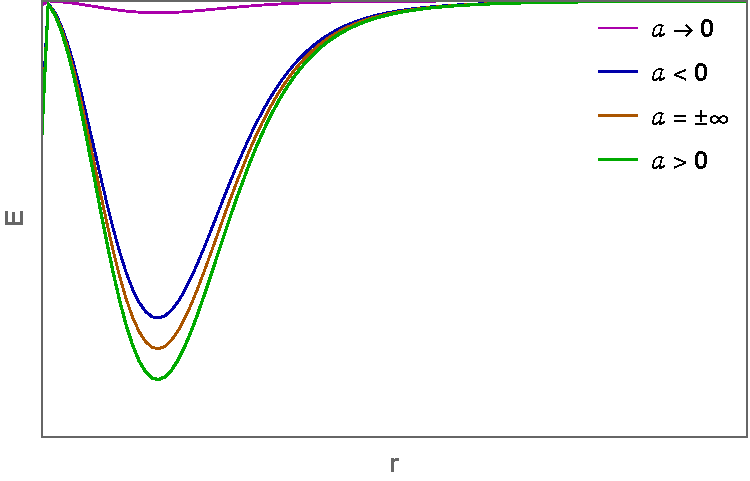
\includegraphics[width=\linewidth]{potential_depth.pdf}
	\caption{The three lowest curves correspond to the potentials used in \Cref{fig:intercept}. As the magnitude of a negative $a$ increases, the potential becomes more attractive until it reaches a constant depth at $a=\pm\infty$. After the change in sign, a further increase of $a$ will instead have a repulsive effect on the interaction.}
	\label{fig:potential_depth}
\end{figure}

\begin{figure}
	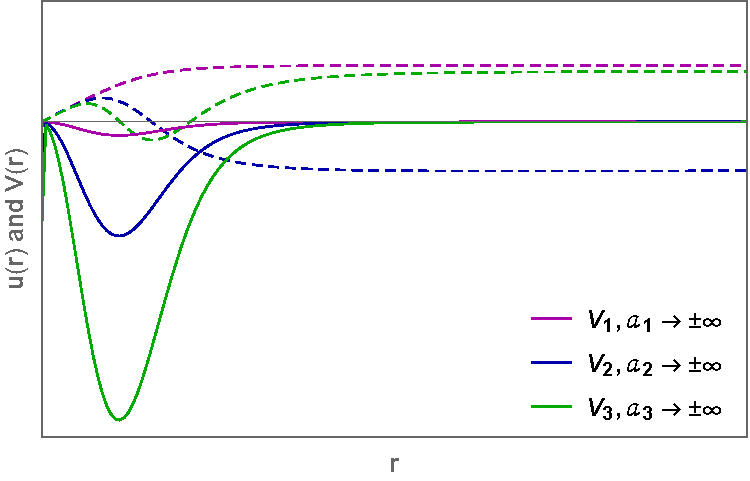
\includegraphics[width=\linewidth]{scattapp.pdf}
	\caption{Illustration of three potentials and their corresponding radial wave functions (the dashed curves).}
	\label{fig:scattapp}
\end{figure}

Positive scattering lengths thus correspond to repulsive effective interactions, which means that the interaction can appear repulsive even in the case of an underlying attractive two-body interaction.